\section{The model}\label{sec:model}

This section describes the agent-based model that carries the contract of Section~\ref{sec:contract} into a
population of households, in the order of the ODD protocol \cite{grimm}. Every statement below is read from
the simulation code. All parameter values and sources are in Appendix~\ref{app:parameters}.
Table~\ref{tab:onepage} first gives the whole model on one page: its objective, its assumptions,
the agents, their state, the control parameters, the dynamics, what each agent optimises, the remaining
equations and what emerges.

\begin{table}[p]
\centering\footnotesize
\caption{The model on one page.}\label{tab:onepage}
\begin{tabularx}{\textwidth}{@{}p{0.17\textwidth}X@{}}
\toprule
Objective & To find whether a payment money whose holders pay a small holding charge, a demurrage, can fund one pooled liquidity
  buffer that lends to its own users without collateral; whether that pool forms and persists with no outside
  support; and who gains or loses against banks and cards and against best-case DeFi. \\
\addlinespace
Assumptions & (i) Total spending is fixed; there is no production and no growth.
  (ii) The pool sees a borrower's expected receipts, lends a bridge only up to what they repay, collects a due
  bridge from all the borrower's money, and a debt survives leaving the network; nobody who can pay chooses not to.
  (iii) A DeFi loan needs collateral worth more than the loan, so it covers no shortfall.
  (iv) People act on their own last month and last year and form no forecast.
  (v) Savers enter on the pool's published quote, the quote rule; a second map has them enter on its realised
  return, the record rule.
  (vi) The reserve rate is constant within a run, and outside deposit and loan rates follow it.
  (vii) The five arrangements face the same people and the same random draws. \\
\addlinespace
Agents and network & People, each one consumer unit, who pay and are paid, hold money, borrow and may own pool
  shares. Three collective entities: the pool, the issuer of P and the outside lenders. People are joined by a
  payment network: each pays one wage to one other person, fixed for the run, and makes 32 service purchases a
  month from sellers drawn afresh each month, uniformly over everyone else, so one person's spending is other
  people's income. Section~\ref{sec:robustness} replaces the uniform draw by a ring and by hub sellers. \\
\addlinespace
State variables & Of a person: bank money $E$, P once in the network, outside savings, pool shares, invoices
  receivable and payable, card balance and loans, and whether it is in the network. Its fixed traits are its
  spending weight, billing and pay cycles, the one wage it pays, its card, score and line. In aggregate:
  participation $A$; pool capital $N$ and its target $N^{*}$; the pool's term book $T$, bridge book $B$ and cash $C$;
  wallet balances $\cyc W$, bridging $\cyc B$ and standby cash $\cyc S$ over a cycle; the learned loss rates
  $\ell_{k}$. \\
\addlinespace
Control parameters & The reserve rate $\rho$, launch participation $a_{0}$ and the extra layoff rate of the
  distress year. The first and third are the environment and the second is the condition a launch starts from. The
  design is the contract, the same in every cell and compared across five arrangements. \\
\addlinespace
Dynamics & \emph{Each day} the payments due settle together, as the fixed point $\sigma = F(\sigma)$ of the shares each
  payer completes (Proposition~\ref{prop:settlement}).
  \emph{Each month} every person re-chooses a cash buffer; a person outside joins with chance
  $\xi_{0} + \xi_{1}s_{i}$, where $s_{i}$ is the share of its trading partners in the network; members, owners
  and savers review leaving, exit~\eqref{eq:exit} and entry with chance $\upsilon$; and the pool sets its coupon,
  charge, target and quote from the cycle just closed.
  \emph{In aggregate} participation follows $A_{t+1} = A_{t} + (j_{0} + j_{1}A_{t})(1 - A_{t}) - \lambda A_{t}$
  \eqref{eq:diffusion} and capital returns to $N = \max(N^{*}, N^{-})$ at each dealing when offers exceed the room
  \eqref{eq:capital}. Section~\ref{sec:laws} writes the laws of motion of the aggregate state, \eqref{eq:law-A} to
  \eqref{eq:law-W}, month by month and in continuous time. \\
\addlinespace
Objective functions & No agent optimises over the world.
  \emph{A person} keeps the cash buffer, from a fixed grid, that would have cost it least over its own last month:
  return given up, credit cost, fees and failure fees.
  \emph{A member} leaves with a logistic probability in its own experienced gain over the last year;
  \emph{an owner} files to redeem by~\eqref{eq:exit} on its realised return against its alternative;
  \emph{a saver} offers its money when the quote $q(N^{*})$ is at least its alternative.
  \emph{The pool} maximises nothing: its prices solve zero-profit and free-entry conditions, the coupon
  $r_{k} = a + o + f + \ell_{k}$ \eqref{eq:coupon}, the demurrage rate $c = \min(K/\cyc W,\, p)$ \eqref{eq:charge} and the
  quote $q(N^{*}) = a$ \eqref{eq:quote}. \\
\addlinespace
Further equations & The cost of the liquidity kept ready, $K = a\,\cyc B + (a - p)\,\cyc S$ \eqref{eq:cost}; the
  bridge price $r_{b} = r_{g} - \kappa a$ \eqref{eq:bridgeprice}; the wallet yield $y = p - c$ \eqref{eq:yield};
  the capital target $N^{*} = T^{\mathrm{need}} + B^{\max}$ \eqref{eq:target}. From them, the size of the demurrage,
  $c/a = \cyc B/\cyc W + (1 - p/a)\,\cyc S/\cyc W$ (Proposition~\ref{prop:size}), and the lending a pool needs to
  carry its fixed cost, $L_{0} \ge \Phi/(r_{\mathrm{ext}} - a - o - \ell)$ (Proposition~\ref{prop:threshold}). \\
\addlinespace
Emergence & Nothing below is set; each arises from the decisions above and the contract applied to what they
  produce. Participation $A$ and its path; pool capital and whether it holds its target, $N/N^{*}$; the coupons,
  the demurrage rate $c$, the bridge price $r_{b}$ and demurrage's share $\theta$ of bridging finance; the share
  of payments that fail; each person's gain against the bank arrangement and against best-case DeFi; and, under
  distress, a run on the pool when owners file to leave after a write-off. These are the order parameters, each
  defined in Section~\ref{sec:measurement}. \\
\bottomrule
\end{tabularx}
\end{table}

\subsection{Purpose and patterns}

The model asks whether a payment money whose holders pay a small holding charge can fund one pooled liquidity
buffer that lends to its own users, whether that pool forms and persists without outside support, and who gains or
loses against today's arrangements. It plays the same simulated people, with the same random events, through five
arrangements (Table~\ref{tab:arms}), so any difference between two arrangements for one person comes from the
arrangement alone. Best-case DeFi gives stablecoin payments and a yield on balances, and no credit to a payer who
is short, since its loan needs collateral worth more than the loan. The pool without
the charge is CPM's contract with the charge set to zero. Nothing then pays for cash standing by, so
its capital target is the average lending need with no peak \eqref{eq:target}. CPM against it therefore shows
what demurrage and the liquidity it pays for add together.

The model compares designs and forecasts nothing. No output predicts a quantity in the United States
economy. The patterns below check the bank arrangement (banks and cards) against data; the new arrangements do not exist to be
checked. The theory of Section~\ref{sec:implications} is the minimal model, written in a few aggregate
quantities. The simulation adds what that theory averages over: people who differ and a network of payments. It also adds
the detail of cards, fees and credit lines that prices today's alternative, since a gain measured against a cheaper
alternative than people have would not be a gain.

Total spending is fixed and there is no production, so the model compares how the same spending is paid and
financed. It is checked against a few patterns and is not fitted to them: the stock of jobs
without a wage under normal job loss (about 1.9\% of jobs, against about 2.0\% of US payroll jobs in 2026), the
tier mix of card holders and their lines against the CFPB's card market report, the scale of the distress year
against the fall in US wages in 2009, and holders' use of cash advances, which runs above the US level and is
allowed for by the cash-advance bound of Section~\ref{sec:measurement}.

\subsection{Entities, state variables and scales}

The agents are people, each standing for one US consumer unit. A person holds bank money $E$, and once in the
network P (USDC in best-case DeFi); one-month outside savings; pool shares valued at net asset value; invoices
receivable and payable; card balances; and loans by lender and kind (pool and outside bridges, instalment loans,
revolving card balances, cash advances, charged-off card balances, rounding overdrafts at a fixed outside rate and
interest-free failure-fee debt). Fixed traits drawn at the start are spending weight, billing cycle and phase, the
one other person it pays a wage to, the pay period and phase of that job, card holding, credit score, card line and
starting balance, whether its income is business receipts, and whether it holds earned-wage access. Net financial
wealth is money, savings, shares and receivables less payables, card balances and every loan; illiquid wealth and a
card's starting balance are outside it.

Three collective entities hold state. The pool holds its cash, its loan book (bridge book $B$, term book $T$), its
standby cash $S$ and its capital $N$, owned by households alone, against its target $N^{*}$. The issuer holds the
reserves behind all P, keeps its custody cost and owns no shares. Outside lenders, card networks, the conversion
provider, the pool's operating provider, validators and the issuer sit outside the household economy and hold no
state beyond the flows recorded with them.

Money is measured in months of mean consumer-unit spending, one unit being \$6,440. Time runs in days of a 30-day
month. A run is a burn-in of six months under the bank arrangement, shared exactly by every arrangement, followed by
60 months after launch. The pool forms by free entry from the first dealing with a lending need. The confirmation
maps and the final development map use 4,000 people; development checks used 1,000.

Figure~\ref{fig:wagenet} draws the wage links of one population. Each person pays one wage to one other person, so
the links form long chains and branches, and a wage that fails has one path onward.

\begin{figure}[htbp]\centering
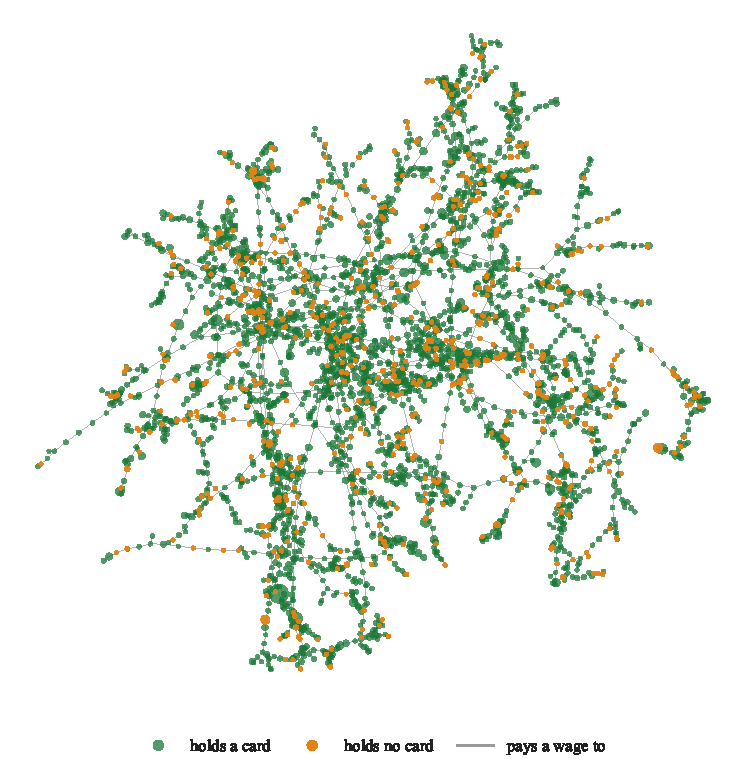
\includegraphics[width=0.8\linewidth]{figures/fig_wage_network.pdf}
\caption{The wage network of one population draw: \NumPeople{} people at the first confirmation seed. Each person
pays one wage to one other person. A node's area follows the person's spending. Purchases, which link each person
to many sellers a month, are not drawn.}
\label{fig:wagenet}
\end{figure}

\subsection{Process overview and scheduling}

Each month runs in this order.
\begin{enumerate}[leftmargin=*,itemsep=1pt]
\item At the launch month only, people are drawn into the network with probability $a_{0}$ and convert their bank
money into P at one conversion fee.
\item Jobs are laid off at the normal rate, plus the distress control's extra rate in the distress year; the month's
service purchases, wage accruals and instalment-credit requests are created.
\item The pool publishes its terms from the last two completed months: the bridge and term coupons, the capital
target $N^{*}$ and the quote at it, the holding charge $c$, its coverage $\kappa$ and the yield on P.
\item Dealing: outside savings mature into cash; owners who review may file to exit and due exits are paid; what is
already due is collected, then overdue wages, then every debt, all from all money; each person chooses a cash buffer
by replaying its own last month; spare money is split into pool offers and outside savings.
\item Thirty days of settlement. Each day: earned-wage accrual; arrears flags; instalments falling due, collected
from all cash and same-day savings; instalment purchases settling that day; the day's bills and wages, with
bridging, cash advances, earned-wage advances and failures; on day 20 the card statement, its minimum payment and
any late fee; the day's own cash flow is recorded for next month's replay; what is due is collected from all money
(missed instalments, then outside bridges dearest first, then pool bridges); overdue wages and then other debts are
repaid from money above the buffer; interest and the pool's operating cost accrue; pool loans 90 days past due are
written down; cards 180 days past due are charged off.
\item The month's card purchases are billed on the statement due on day 20 of the next month.
\item Close: savings earn their rate; the reserve return on P pays wallet holders their yield net of the charge and
pays the charge and the pool cash's return to the pool; the pool pays its fixed cost, its value per share and the
owners' realised return are set, and the month is entered in the record the next terms read; experience of using
the network is computed; people leave and join; card rewards are paid; durables depreciate; consumer prices deflate
every nominal stock; next month's spending is set; records are written.
\end{enumerate}

\subsection{Time and updating}\label{sec:updating}

The clock is the day, the same for every population size. No rule visits people one after another and none draws a
visiting order: every rule applies to all people in one step, and chance enters as an independent draw for each
person. Results can depend on the update scheme, a known hazard of agent-based models
\cite{huberman,axtell}, so the scheme is stated here and tested in Section~\ref{sec:robustness}. Three kinds of event
update in three ways.

\emph{Calendar events} fall on dates that contracts set: wages on each job's pay dates, bills on each seller's
billing date, instalments on the borrower's billing date, the card statement on day 20, the pool's terms at the
start of a month. Cycles of 1, 7, 15, 30 and 60 days on random phases spread these dates over the month, so people
are not in step. A monthly calendar with a fixed sequence of markets is the common choice in such models
\cite{baptista,poledna}. Within a day the pool's cash goes first to instalment purchases, then to bridges and, on
day 20, to card statements, pro rata to requests within each.

\emph{Decisions} are reviewed monthly. Leaving, owners' exit and savers' entry are each reviewed by a random part
of the people concerned, a person with chance $\upsilon = 1 - e^{-0.166}$ a month. That is the exact monthly chance
of a review clock that rings at rate 0.166 \cite{gillespie}, so these are random asynchronous updates at
monthly resolution. Joining is a chance of at most 3.4\% a month for each person outside. Leaving and joining
read the month's participation before either is applied. One decision is taken by everyone in the same dealing:
the cash buffer, chosen by the rule given under adaptation in the design concepts below.
Section~\ref{sec:robustness} repeats the runs with only a random part of the population
re-choosing its buffer each month. The diffusion equation \eqref{eq:diffusion} and the contract's identities are
written month by month, on the model's own clock.

\emph{Settlement} of a day's payments is simultaneous, because what a payer can pay depends on what it is paid
that day. Let $\sigma_{i}\in[0,1]$ be the share of its payments due on a day that payer $i$ completes, and $F$ the day's
map from every payer's share to the shares their receipts then allow. Cover is taken in the fixed order of the
submodel below and the pool's queue is held fixed. The day's outcome is a fixed point $\sigma = F(\sigma)$, found by repeating
$F$ from $\sigma = 1$ until no share moves by more than $10^{-14}$.

\begin{proposition}[Settlement]\label{prop:settlement}
(i) On a day on which the pool's cash covers every request it admits, and on every day in the arrangements without
a pool, $F$ is monotone, and the iteration from $\sigma = 1$ stops at the greatest fixed point of $F$.
(ii) With the day's credit taken as given, the fixed point is unique if and only if no set of payers completes a
positive share while its members have no means of their own that day and are paid that day only by one another.
Such a set pays only its own members.
(iii) With the day's credit taken as given, settlement one payer at a time in any order, each paying what it can
across its payments as money arrives until nothing more can be paid, ends at the least fixed point, and so at the
same outcome as the simultaneous solution whenever (ii) gives uniqueness.
\end{proposition}

\begin{proof}[Sketch]
(i) Receipts do not fall when any payer's share rises, and a payer's shortfall does not rise with its receipts. The
part of a shortfall left after each source of cover does not fall as the shortfall rises: savings, the cash advance
and earned-wage access are capped amounts, and the pool lends the largest draw that its receipts test admits for
that draw and every smaller one, which leaves an unlent part that cannot fall (a test checks this over the test's
parameter ranges). So $F$ is monotone. From $F(1)\le 1$ the iterates fall, and they stay above every fixed point
$g$, since $g = F^{k}(g) \le F^{k}(1)$; the point at which they stop is therefore the greatest.
(ii) With means $m_{i}$, dues $d_{i}$ and receipts $R_{i}(\sigma)$, the map is $F_{i}(\sigma) = \min\{1, (m_{i} +
R_{i}(\sigma))/d_{i}\}$. Let $\sigma$ be the greatest fixed point, $\sigma'$ another, and $D$ the payers with
$\sigma_{i} > \sigma'_{i}$. Each member of $D$ pays all it has under $\sigma'$, so
$d_{i}(\sigma_{i} - \sigma'_{i}) \le R_{i}(\sigma) - R_{i}(\sigma')$, and the right side is
what members of $D$ pay $i$ more under $\sigma$. Summing over $D$, the extra paid by $D$ is at most the extra $D$ pays
to its own members, which is at most the extra paid by $D$. Equality throughout means $D$ pays only its own
members; summing what its members pay under $\sigma'$ then gives that their means and their receipts from outside $D$
are zero. Conversely, the shares of such a set can be scaled down together and remain a fixed point.
(iii) By induction no payer's cumulative payment exceeds what it pays at the least fixed point, and where the
process ends no payer can pay more, which is a fixed point.
\end{proof}

Part (i) is the fictitious default algorithm of \cite{eisenbergnoe}: the payers who fail in its first round would
fail even if paid in full, and the rest fail because others did \cite{elsinger}. Part (ii) names the one case in
which the simultaneous solution does more than a sequence of payments could: a closed loop of payers without
money, who all pay in the model's solution and none of whom could pay first. Payment systems call that state
gridlock and resolve it by settling the loop at once \cite{bech}. The model's choice is the same in every
arrangement and leans toward completion. Every run records, each day, the payments that rest on it; they are
at most \NettingShareMost{} of completed value in any run (Section~\ref{sec:robustness}). When the pool's cash is short,
requests are served pro rata and $F$ need not be monotone, since a borrower with more receipts can ask for more and
cut every other borrower's share. The code detects two states that repeat and defers, for the day, the request
admitted in one and refused in the other. Within a day money received can be paid on, and the day has no
earlier and later; this too is the same in every arrangement.

\subsection{Design concepts}

\emph{Emergence.} Participation, pool capital, the coupons, the holding charge and failed payments are not set; they
arise from individual buffer, joining, leaving, entry and exit decisions and from the pool's rules applied to what
those decisions produce. The demurrage rate is computed each month from the bridging and standby cash the
pool kept ready over the last two months and from the wallet P balance $W$ held over them. Participation $A$ is
the share of people in the network during each month, before its month-end joining and leaving.

\emph{Adaptation.} People follow their own experience and do not optimise over the world. A person keeps the cash
buffer, from a fixed grid of multiples of its own spending, that would have cost least had it faced its own last
month again, counting the return given up, credit cost, cash-advance and earned-wage fees and failure fees. For a
member with no shortfall in that month the choice also reads the share of requests the pool served. A
member reviews its membership with the monthly chance $\upsilon$ of Section~\ref{sec:updating} and leaves with a logistic
probability that its average monthly experience over the last year falls short of one conversion of its average P
balance spread over that year. Owners review on the same rule with their own realised return against their
alternative. Savers review entry with the same probability and offer their money-market part when the pool's
published quote is at least their alternative.

\emph{Interaction.} People interact through the payment network: one person's spending is other people's income,
so a failed or late payment is missing income for its payee on that day. They also interact through the pool, whose
cash is rationed pro rata among borrowers on a day, and through joining, which rises with the share of a person's
own counterparties in the month who already use the network.

\emph{Stochasticity and common random numbers.} Each random stream has its own seed: the population's traits, the
job-loss stock at the start, each month's layoffs, purchases, shocks and credit requests, joining and leaving draws,
owners' draws and savers' entry draws. Every stream is drawn in every arrangement and month,
used or not, so all five arrangements see the same numbers. For one seed every arrangement therefore draws the same
population, the same obligations on the same dates and the same job-loss spells. What differs is the arrangement's
rules from launch on and, through them, what people choose: their buffers, participation and borrowing.
Initial wealth is not drawn: it is the mean of each equal quantile band of the Pareto law, so every seed has the same
wealth vector and seeds vary only the economy's events. Within a month one uniform draw per job decides its layoff at
every distress level, so a higher level's layoffs contain a lower level's and every level shares the months before
the distress year.

\emph{Observation.} Each run records monthly aggregates and, by person and month, net wealth, participation, pool
ownership and borrowing, completed and lost purchases, credit by lender, fees and failure counts. The pool's
monthly records include $c$, $\kappa$, the charge's share $\theta$ of bridging finance, $B$, $T$, $W$, $N$ and
$N^{*}$. Arrangements are compared person by person on the same seed.

\subsection{Initialisation}

Initial wealth follows a Pareto law of shape 1.5, scaled so that the median person holds 0.6 months of its own
spending. Spending rises with relative wealth to the power 0.5 and has mean one. Liquid wealth is the lower of that
level and the Fed survey's liquid savings at the same rank (18\% below \$100, 30\% below \$500, half below \$2,000),
up to the 62nd percentile. The rest is illiquid wealth, which counts toward net worth for spending and for each
person's wealth group but never pays a bill. Everyone starts with all liquid wealth as bank money and nothing saved.
Billing cycles are assigned in exact proportion: daily, weekly, fortnightly, monthly or every 60 days, from BLS pay
frequencies for the 58.3\% of receipts that are wages and from settlement patterns for business receipts. Card
ownership follows income bracket in exact proportion, with spending rank as income. A credit score is drawn by a
Gaussian rank link to income from the FICO distribution, and sets the card's APR tier, its line and its starting
balance. Jobs in a spell at the start are drawn from the steady stock of normal job loss. The network is empty until
launch.

\subsection{Input data and calibration}

All calibrated values, with their units and sources, are in Appendix~\ref{app:parameters}. A test checks every
entry of that table against the code. Outside deposit and credit rates follow the outside rate from their October
2026 levels, the same in every arrangement: the savings deposit rate by 0.08 of a change, card and business rates
one for one, and new vehicle and personal loans by 0.75 and 0.63. A loan keeps the rate it was made at. The pool's
fixed cost is a large lending protocol's paid service providers over US consumer units. The experiment varies three
controls: the reserve rate $\rho = r_{\mathrm{out}}$, launch participation $a_{0}$ and the extra layoff rate of the
distress year. Their grid values, the cells they make and the number of seeds are in
Section~\ref{sec:measurement}.

\subsection{Submodels}

\emph{Income, pay days and job loss.} Each person pays 58.3\% of its spending as one wage to one other person drawn
at random, so about $e^{-1} \approx 37\%$ of people receive no wage. It pays the other 41.7\% as 32 service purchases a month to
sellers drawn at random on random days. Wages accrue daily and settle on the job's own pay dates; service bills
settle on the seller's billing date, so receipts arrive in lumps while spending is spread. Every month each job not
already in a spell is laid off with probability 0.55\%, weighted toward lower incomes by unemployment by education
(1.13, 1.09, 1.03 and 0.92 times the average from the lowest income bracket up). The spell is log-normal with a
completed median of 61 days, set so that spells in progress match the BLS median of 11.5 weeks and mean of 24.8
weeks. A job in a spell pays nothing for those days. Unexpected expenses, the other common cause of a shortfall,
are switched off in every run, so shortfalls come from the timing of receipts and payments and from job loss alone.

\emph{Spending and the payment network.} A service purchase is card-eligible with probability 0.671, the share of
service spending that is not housing. A card holder's card-eligible purchase from a seller in the network is paid in
P (USDC in best-case DeFi) when both are in the network and the holder's own money covers that day's payments, at
the gas of one transfer for P and two for USDC. Otherwise it goes on
the card up to the room left on the line, whole purchases smallest first, and the rest is paid like any other bill.
Each day a payer's own money and the day's receipts pay its payments, which settle together as
Section~\ref{sec:updating} sets out.

\emph{Settlement and failed payments.} A payer short on a day uses, in fixed order: its outside savings the same
day; the pool, if it is a member not in arrears and the pool is no dearer than the line it holds; a cash advance on
its card up to its cash line; and earned-wage access up to half of the wages earned and still unpaid. Only then does it
fail. A payer completes the same share of each of its payments that day. A failed service purchase is lost: the
seller receives nothing and the buyer keeps the money. A failed wage stays owed and is re-queued to the job's next
pay date. A failed bill or wage carries a flat \$27 fee, booked as interest-free debt repaid first, at most one a
payer a day and two a month. A failed card-eligible purchase is declined without a fee.

\emph{Cards, lines, minimum payments, cash advances, late fees and charge-off.} Each holder's line is the average
line of its score tier and starts partly used by a fixed outside balance that bears no interest and is never
collected. Purchases are free until the statement is due on day 20 of the next month. The statement is paid from
money and same-day savings, a member's unpaid part may be paid by the pool, and the rest revolves at the card's APR.
A non-card bill reaches the card only as a cash advance, up to 20\% of the line within the room left, at 30\% a
year from the day taken (moving with the outside rate) and a fee of the greater of \$10 or 5\%. The minimum payment
is the greater of \$40 and 1\% of the balance plus the cycle's interest and fees and any amount past due, never
above the balance. Missing it costs \$30, or \$41 for a repeat within six cycles, and makes the card delinquent,
which blocks pool credit. A card 180 days past due is charged off: its line closes and its balance stays owed at no
further interest. Lines are held through the distress year.

\emph{The bank arrangement.} Bank money earns the checking yield. Outside savings earn each person's wealth group's
mix of the savings deposit rate and the money-market rate $\rho$. Instalment requests for vehicles, personal needs
and business are made at sourced rates and sizes, funded first from money above the buffer and then by an outside
lender at a score-based rate, subject to a 43\% debt-to-income limit for households and to not being in arrears for
firms. Instalments fall due on the borrower's first billing date each month. Every bank arrangement rule also runs,
unchanged, in the other four arrangements.

\emph{Best-case DeFi.} Members hold their working balance as USDC, which converts to and from dollars at no fee. It
earns the bill rate less the Sky Savings Rate's observed spread under it, 0.44 point a year, moving one for one with
$\rho$. Payments between members cost two transfers of gas. DeFi's loan requires collateral worth more than the
loan, so a payer who is short has nothing to lock and the loan covers none of its shortfall. No household borrows
from it, and a short member follows the bank arrangement's alternatives.

\emph{Joining and leaving the network.} After launch a person outside joins in a month with probability
$\xi_{0} + \xi_{1} s_{i}$, with $\xi_{0} = 0.03/12$, $\xi_{1} = 0.38/12$ and $s_{i}$ the share of its counterparties
in the month who use the network, and converts its bank money into P at one conversion fee. This is the hazard of
\cite{bass}, innovation plus imitation, with the average coefficients of \cite{sultan}, as quoted by
\cite{vandenbulte}, and with the population
share replaced by the share among the person's own trading partners. Influence that rises in proportion to the
share of a person's contacts who have adopted is what \cite{karsaicontagion} measure for an online service. The
rule is a simple contagion: each contact adds to the chance on its own. A payment money has complements and asks
for trust, the case for a complex contagion, in which a person adopts only once enough of its contacts have
\cite{centolamacy}. Card and mobile payments show such complements in data \cite{higgins,crouzet}. In the
model the complement enters through use and leaving, not through joining: P can be spent only with a seller
who takes it, and a member whose experience falls short leaves. Section~\ref{sec:robustness} replaces the rule by a
threshold rule, with thresholds measured for an online service \cite{karsaicascades} and with one common
threshold \cite{watts}. A member's bank money
receipts join its P without a fee. A member leaves by the experience rule above and redeems its P at one conversion
fee. Shares and debts persist after leaving.

\emph{The pool's lending, dealing and exits.} The pool runs the contract of Section~\ref{sec:contract}. Its coupon
is the owners' alternative $a$ plus the operating cost $o$, the fixed cost $\phi$ spread over last cycle's lending
and the loss rate learned by product. A bridge is sealed at that coupon less the share $\kappa$ of its capital part
that the charge covers. A bridge is lent only up to what the borrower's expected receipts of the next two months
repay after every debt ranked ahead of it. It falls due on the first receipt date that covers it; from then it is
collected from all the borrower's money. Term loans, the instalment loans of the bank arrangement, are offered when
the pool's coupon is no dearer than the
outside rate. Lending is rationed pro rata to the cash new loans may take. Wallet P earns $p$ less the demurrage $c$
on its balance-time and the charge goes to the pool. Savers' offers, made by the entry rule of the design concepts
above, are accepted pro rata up to the target $N^{*}$. An exit executes after two
months at that month's value, from pool cash and the same dealing's new subscriptions. A pool loan 90 days past due
is written down to zero, the debt stays owed and later payments are recoveries. In indexed CPM, P and the pool's
loans are not deflated and the contract runs at the real reserve rate.

\emph{The distress year and where the lost wages go.} In months 25 to 36 after launch the distress control adds an
extra monthly layoff rate per job. A layoff is extra when its draw lies above the normal rate, so the level adds
layoffs without moving the normal ones. After normal job loss the payer keeps the wage and owes nothing. The wage of
an extra layoff leaves the household economy for the whole spell: its payer still owes it on the job's pay dates, to
the outside, and its worker receives nothing. Such a wage is settled by its payer like any wage, fee-bearing when it
fails and re-queued while unpaid, but it is nobody's receipt and never a P payment. No unemployment insurance is
modelled.

\emph{Conservation.} Money moves only between named accounts, and every flow has a payer and a receiver. What
households pay an intermediary outside the economy leaves it and is recorded as an outside flow: interest to outside
lenders, failure fees, the merchant card fee, conversion fees, gas, earned-wage fees, cash-advance and late fees, the
pool's operating and fixed costs, the wages of extra layoffs, and the pool's cash when a pool whose owners have all
left is wound up. What intermediaries pay households enters the same record: savings income, the checking yield,
card rewards, the reserve return paid on wallet P and on the pool's own cash, and DeFi's yield on USDC. The holding
charge is withheld from wallet holders' yield and credited to the pool, so it moves money within the household
economy. Summed over people, the monthly change in net wealth equals the outside flows, plus the write-down and
recovery of pool loans, plus the loss of value of nominal stocks to inflation. The test suite checks this identity
every month in every arrangement to $10^{-12}$ of a month's mean spending. A separate reserve account moves wherever
P is created or destroyed, so the backing of P by reserves is checked, not assumed.

\subsection{The laws of motion}\label{sec:laws}

Summed over people, the model has a small state. This subsection writes its laws month by month and, beside each, in
continuous time, per person and in months of mean spending. In month $t$, $A_{t}$ is the share of people in the
network and $N_{t}$ is pool capital after the dealing that opens the month, as in \eqref{eq:capital}. $T_{t}$,
$B_{t}$ and $C_{t}$ are the term book, the bridge book and pool cash at the close, the books as principal still
carried and cash less any operating bill unpaid. A bar, as in $\bar W_{t}$ for wallet balances, is the average over
the month's days. The learned loss rates $\ell_{k}$ complete the state. Prices rise by $\pi$ a month and the unit of
account is real, so each close divides every nominal stock by $1+\pi$ (indexed CPM leaves P and the pool's loans
undivided). The continuous forms are written for $\pi = 0$.
\begin{equation}
A_{t+1} = A_{t} + A^{\mathrm{in}}_{t} - A^{\mathrm{out}}_{t},
\qquad
\frac{\mathrm{d}A}{\mathrm{d}t} = (j_{0} + j_{1}A)(1 - A) - \lambda A .
\label{eq:law-A}
\end{equation}
People join and leave at the close, so the first form is an identity: $A^{\mathrm{in}}_{t}$ and
$A^{\mathrm{out}}_{t}$ are the shares of people who join and who leave by the rules of the submodels. The second is
its mean field, \eqref{eq:diffusion} in continuous time: every contact share is replaced by $A$ and the leaving rule
by one realised rate $\lambda$.
\begin{equation}
(1+\pi)\,T_{t} = T_{t-1} + T^{\mathrm{new}}_{t} - T^{\mathrm{rep}}_{t} - T^{\mathrm{off}}_{t},
\qquad
\frac{\mathrm{d}T}{\mathrm{d}t} = T^{\mathrm{new}} - \sum_{M}\frac{1}{M}\int_{0}^{M} T^{\mathrm{new}}_{M}(t-u)\,\mathrm{d}u - T^{\mathrm{off}} ,
\label{eq:law-T}
\end{equation}
\begin{equation}
(1+\pi)\,B_{t} = B_{t-1} + B^{\mathrm{new}}_{t} - B^{\mathrm{rep}}_{t} - B^{\mathrm{off}}_{t},
\qquad
\frac{\mathrm{d}B}{\mathrm{d}t} = B^{\mathrm{new}} - \int_{0}^{5} B^{\mathrm{new}}(t-u)\,\mathrm{d}G(u) .
\label{eq:law-B}
\end{equation}
The first forms are identities in principal: new lending, less principal collected, less principal written down
ninety days past due. New lending is a named flow: $T^{\mathrm{new}}$ is the instalment credit members take from the
pool while its term coupon is no dearer than the outside rate, $B^{\mathrm{new}}$ the shortfalls the pool bridges,
both rationed by the cash new loans may take. A term loan repays its principal in $M$ equal monthly
instalments, 60, 24 or 11 by product, and is never prepaid, which gives the delay in \eqref{eq:law-T}, exact when no
instalment is missed. A bridge falls due on its covering date, within two months, and is written down ninety days
later, so it leaves the book within five months. $G(u)$ is the share that has left $u$ months after the draw. It
comes from the covering-date rule and repayment out of money above the buffer; fixing it is an approximation.
\begin{equation}
N_{t+1} = \frac{(1+R_{t})\,N_{t}}{1+\pi} + N^{\mathrm{in}}_{t+1} - N^{\mathrm{out}}_{t+1},
\qquad
\frac{\mathrm{d}N}{\mathrm{d}t} = R\,N + N^{\mathrm{in}}(t) - N^{\mathrm{out}}(t) .
\label{eq:law-N}
\end{equation}
$N^{\mathrm{in}}$ is the subscriptions accepted and $N^{\mathrm{out}}$ the redemptions paid at a dealing, both at net
asset value, so both forms are identities. The test suite recomputes \eqref{eq:law-N} from the stored monthly
records of the development map and finds it to rounding in every month of every run. $R_{t}$ is the month's realised return, and $R_{t}N_{t}$ the income
statement in the proof of Proposition~\ref{prop:fair}: coupons accrued, the charge $c_{t}\bar W_{t}$ and
$p\,\bar C_{t}$ on cash, less $o\,\bar L_{t}$, the fixed cost $\Phi_{t}$ and write-downs net of recoveries. The delay
sits in $N^{\mathrm{out}}$: what is paid at $t$ was filed at $t-\delta$ or earlier, with $\delta$ the notice of two
months, and filing follows \eqref{eq:exit}. In the mean field it is, before lapses and rationing, the review rate
times the capital-weighted mean of \eqref{eq:exit} times $N(t-\delta)$. Subscriptions are the lesser of the money
offered and the room, so when offers exceed the room \eqref{eq:law-N} reduces to \eqref{eq:capital}.
\begin{equation}
(1+\pi)\,C_{t} = C_{t-1} + N^{\mathrm{in}}_{t} - N^{\mathrm{out}}_{t} - T^{\mathrm{new}}_{t} - B^{\mathrm{new}}_{t}
 + Y_{t} - o\,\bar L_{t} - \Phi_{t} + c_{t}\,\bar W_{t} + p\,\bar C_{t} .
\label{eq:law-C}
\end{equation}
$Y_{t}$ is the money collected from borrowers: principal, coupons and recoveries. Every term is a movement of pool
cash in the ledger, so \eqref{eq:law-C} is an identity; in continuous time its left side is
$\mathrm{d}C/\mathrm{d}t$, with no delay of its own. The four pool laws are not independent: with $I_{t}$ the
coupons accrued and not yet collected, the balance sheet at each close is $T_{t}+B_{t}+C_{t}+I_{t} =
(1+R_{t})N_{t}/(1+\pi)$.
\begin{equation}
\bar W_{t} = A_{t}\,w_{t} .
\label{eq:law-W}
\end{equation}
A member holds all its working money as P and a person outside holds none, so with $w_{t}$ the mean money of a
member over the month \eqref{eq:law-W} is an identity. Wallet balances are not a free state: $w_{t}$ comes from each
member's buffer rule and the daily settlement and has no closed form.

The contract closes the system. Each month it reads the two months before: the sums $\cyc B = \bar B_{t-1}+\bar
B_{t-2}$, $\cyc W$ and $\cyc L$, and from the daily paths of bridging and cash the peak \eqref{eq:peak} and the
standby \eqref{eq:standby}. It returns the coupons \eqref{eq:coupon} with \eqref{eq:fixed}, the charge, the bridge
price and the yield \eqref{eq:cost} to \eqref{eq:yield}, and the target and the quote \eqref{eq:target} and
\eqref{eq:quote}. The loss rates follow \eqref{eq:loss}, with its lag of three months. These terms act on the named
flows: the coupons on new lending, the yield and the loan prices on members' experience and so on
$A^{\mathrm{out}}$, the quote on $N^{\mathrm{in}}$, the realised return on $N^{\mathrm{out}}$. Individual behaviour
enters through those flows, $w_{t}$ and $G$. The whole is a delay system, with lags of two months (observation),
two (notice), three (loss recognition), twelve (the experience behind leaving and exit) and the lives of the loans.
